\chapter{Trabajo Relacionado}
\label{champ:relatedwork}
\bigskip
\barra
\bigskip

\section{Redes porosas sujetas al Principio de Construcción}
Existen varios algoritmos para la creación de redes porosas que siguen el MDSE y que solo están sujetos al $PC$. Entre ellos están BiaSED\cite{ref1} y NoMISS\cite{ref3} y sus respectivas versiones paralelas descritas en \cite{ref4}, estos algoritmos destacan debido a que permiten crear redes porosas de gran tamaño. En este capítulo se presentara el comportamiento de dichos algoritmos de manera breve y concisa.\\

\subsection{Algoritmos Secuenciales}
\label{subsec:seqversions}
En esta sección se presentan dos algoritmo secuenciales para la creación de redes porosas sujetas únicamente al $PC$, en estas versiones la primera únicamente hace uso del Método de Monte Carlo \cite{ref15} y la segunda se basa un algoritmo voraz que logra un mayor rendimiento y escalabilidad.\\

\subsubsection{Algoritmo BiaSED}
\label{subsubsec:biased}
El algoritmo BiaSED (Biased Simulation Early Design) se describe completamente en \cite{ref1} y \cite{ref4}. Se define como un algoritmo iterativo que se compone de tres pasos fundamentales. En el primer paso, se generan aleatoriamente los tamaños de los sitios y los enlaces (en base a las distribuciones $F_S(R_S)$ and $F_B(R_B)$) y son asignados al azar dentro de la red porosa. La inserción se repite hasta que que la red este completamente inicializada. El resultado de este primer paso es una red porosa que probablemente no cumpla con el $PC$, especialmente cuando hay un alto traslape entre $F_S(R_S)$ y $F_B(R_B)$.\\

El segundo es la ejecución de una serie de Pasos de Monte Carlo ($MCs$) hasta que se genera una red válida que cumple con el $PC$. Un paso de Monte Carlo involucra $4L^3$ intercambios de tamaños de poros, lo anterior para lograr que las conexiones entre los poros sean válidas. Cada uno de los intercambios se hace cambiando el tamaño de dos sitios o enlaces, los cuales se seleccionan aleatoriamente; un intercambio es válido si y solo si el número de violaciones al $PC$ es menor o igual al número de violaciones al $PC$ existentes antes del intercambio, de lo contrario el intercambio es rechazado.\\

\subsubsection{Algoritmo NoMISS}
\label{subsubsec:nomiss}
NoMISS (No Mistake Initial Seeding Situation) es un algoritmo voraz que trabaja con pequeñas soluciones válidas y que a través de iteraciones llega a una solución válida completa, este algoritmo se describe completamente en \cite{ref3}. El método se puede separar en tres pasos fundamentales:

\begin{enumerate}
\item \textbf{Generación de Poros}: se crean las listas de sitios $L_{S}$ y $L_{SC}$, los radios de los sitios de forma aleatoria (en base a la distribución $F_S(R_S)$), los sitios se ordenan de forma ascendente y se almacenan en la lista etiquetada como $L_{S}$. Entonces se generan los radios de los enlaces  de forma aleatoria (en base a la distribución $F_B(R_B)$); por cada enlace generado, este se intenta conectar al primer sitio de la lista $L_{S}$ mientras se cumpla el $PC$. Si no es posible, el enlace se intenta conectar con el siguiente sitio en $L_{S}$, y así sucesivamente hasta que la conexión cumpla el $PC$. Cada vez que un sitio en $L_{S}$ completa su contorno es decir tiene $C=6$ enlaces conectados, el sitios es trasladado a la lista etiquetada como $L_{SC}$. $L_{SC}$ contiene sitios con sus respectivos seis enlaces válidos y en $L_{S}$ contiene sitios con conexiones incompletas. Todos los enlaces conectados tanto $L_{SC}$ como $L_{S}$ siempre cumplen el $PC$.\\

\item \textbf{Sembrado}: en este paso se elijen $k$ semillas (es decir $k$ sitios) de forma aleatoria de la lista $L_{SC}$, y son insertados en posiciones aleatoria de la red, entonces los otros sitios de $L_{S}$ son insertados alrededor de cada semilla, generando así estructuras cúbicas hasta logar el tamaño establecido como cluster-size, en la Figura \ref{fig:cluster_nomiss}  se muestra la construcción de un cluster de tamaño 3x3x3. Cuando un sitio es conectado a otros sito en un cluster, solo se necesita de un enlace para su conexión (y debe de cumplir con el $PC$). El enlace sobrante es asignado a otro sitio en $L_{S}$, siguiendo el mismo procedimiento del Paso 1.\\

\item \textbf{Rellenado}: una vez terminado el proceso de siembra se comienza el rellenado de los espacios vacíos de la red esto se realiza seleccionando aleatoriamente una de las semillas iniciales y se hace crecer su cluster hasta que se ocupen todos los espacios vacíos de la red.
\end{enumerate}

\begin{figure}[hbtp]
\centering
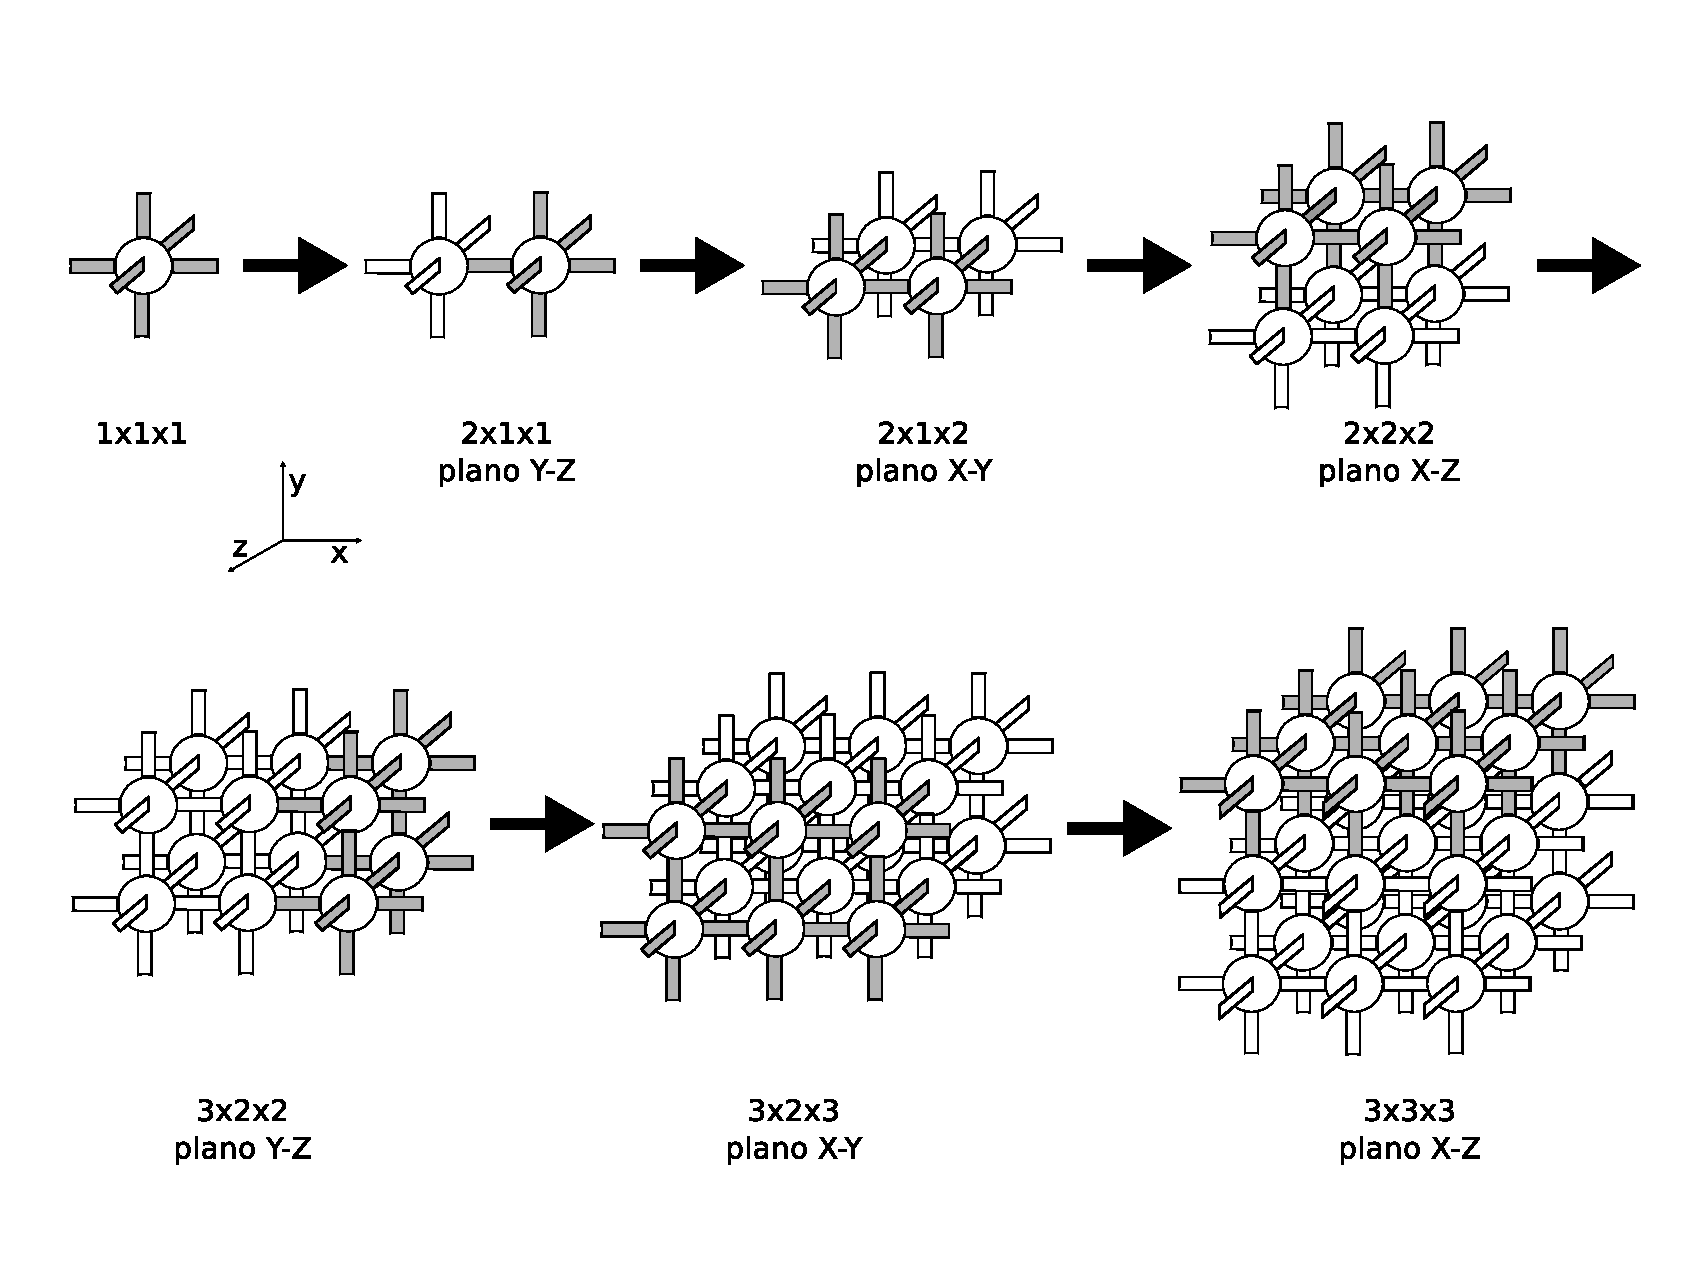
\includegraphics[width=5.0in]{img/cluster-nomiss_es.pdf}
\caption{Construcción de un cluster con NoMISS de tamaño 3x3x3}
\label{fig:cluster_nomiss}
\end{figure}

El Algoritmo NoMISS a diferencia del BiaSED, no hace uso de $MCs$ para crear desde el inicio una red porosa válida.\\

\subsubsection{Otros Algoritmos}
En \cite{ref5} se muestra una primera aproximación para la creación de redes porosas las cuales cumpliesen completamente con el $PC$ y las $RG$; sin embargo el método propuesto resulto en una solución impráctica ya que requería de grandes tiempos de ejecución para la generación de redes porosas de tamaños relativamente pequeños(que contenían a lo más $40^3$ poros).


\subsection{Algoritmos Paralelos}
\label{subsec:algspar}
En esta sección se presenta una descripción breve de algunos algoritmos paralelos que se encuentran descritos a detalle en \cite{ref4} están diseñados para trabajar a través de Paso de Mensajes utilizando la tecnología de Message Passing Interface(MPI), en cada versión paralela la red se divide en pequeñas subredes como se observa en la Figura \ref{fig:distribucion_rw}, esta división se hace en base al número de nodos a utilizar, cada nodo tiene una subred de tamaño $L_x \cdot L_y \cdot L_z$ dicha distribución se hace utilizando funciones especificas de MPI. Los nodos mantienen una topología tipo toro, esto para crear una interconexión entre las distintas subredes. Para la explicación de los algoritmos es establece que un nodo es un proceso MPI.

\subsubsection{Algoritmo Paralelo BiaSED}
\label{subsubsec:pbiased}
El algoritmo paralelo BiaSED se describe completamente en \cite{ref4}, tal y como se comento al inicio de este capítulo la red porosa se divide en subredes las cuales se distribuyen entre los nodos de un cluster utilizando la tecnología de MPI, en la Figura \ref{fig:distribucion_rw} se muestra como se distribuye una red entre nodos. A continuación se describen a grandes rasgos los pasos de esta algoritmo:

\begin{enumerate}
\item Cada nodo generará $L^3/N$ sitios y $3L^3/N$ enlaces, donde $N$ es el número de nodos a utilizar, cada nodo ejecuta el paso uno del algoritmo secuencial

\item Lo siguiente es ejecutar $4L^3/N$ $MCs$ sobre cada subred a esto se le llama $MCs$ paralelo, esto proceso se realiza excluyendo a los sitios de las caras exteriores de la subred

\item Para que cada poro tenga la posibilidad de intercambiarse con otro de una subred distinta, se realizan una serie de transferencias parciales entre los nodos vecinos de cada subred

\item Repetir los pasos 2 y 3, alternando los ejes $x$, $y$ y $z$. Después de un número de $MCs$ paralelos se obtiene una red porosa válida
\end{enumerate}

\begin{figure}[hbtp]
\centering
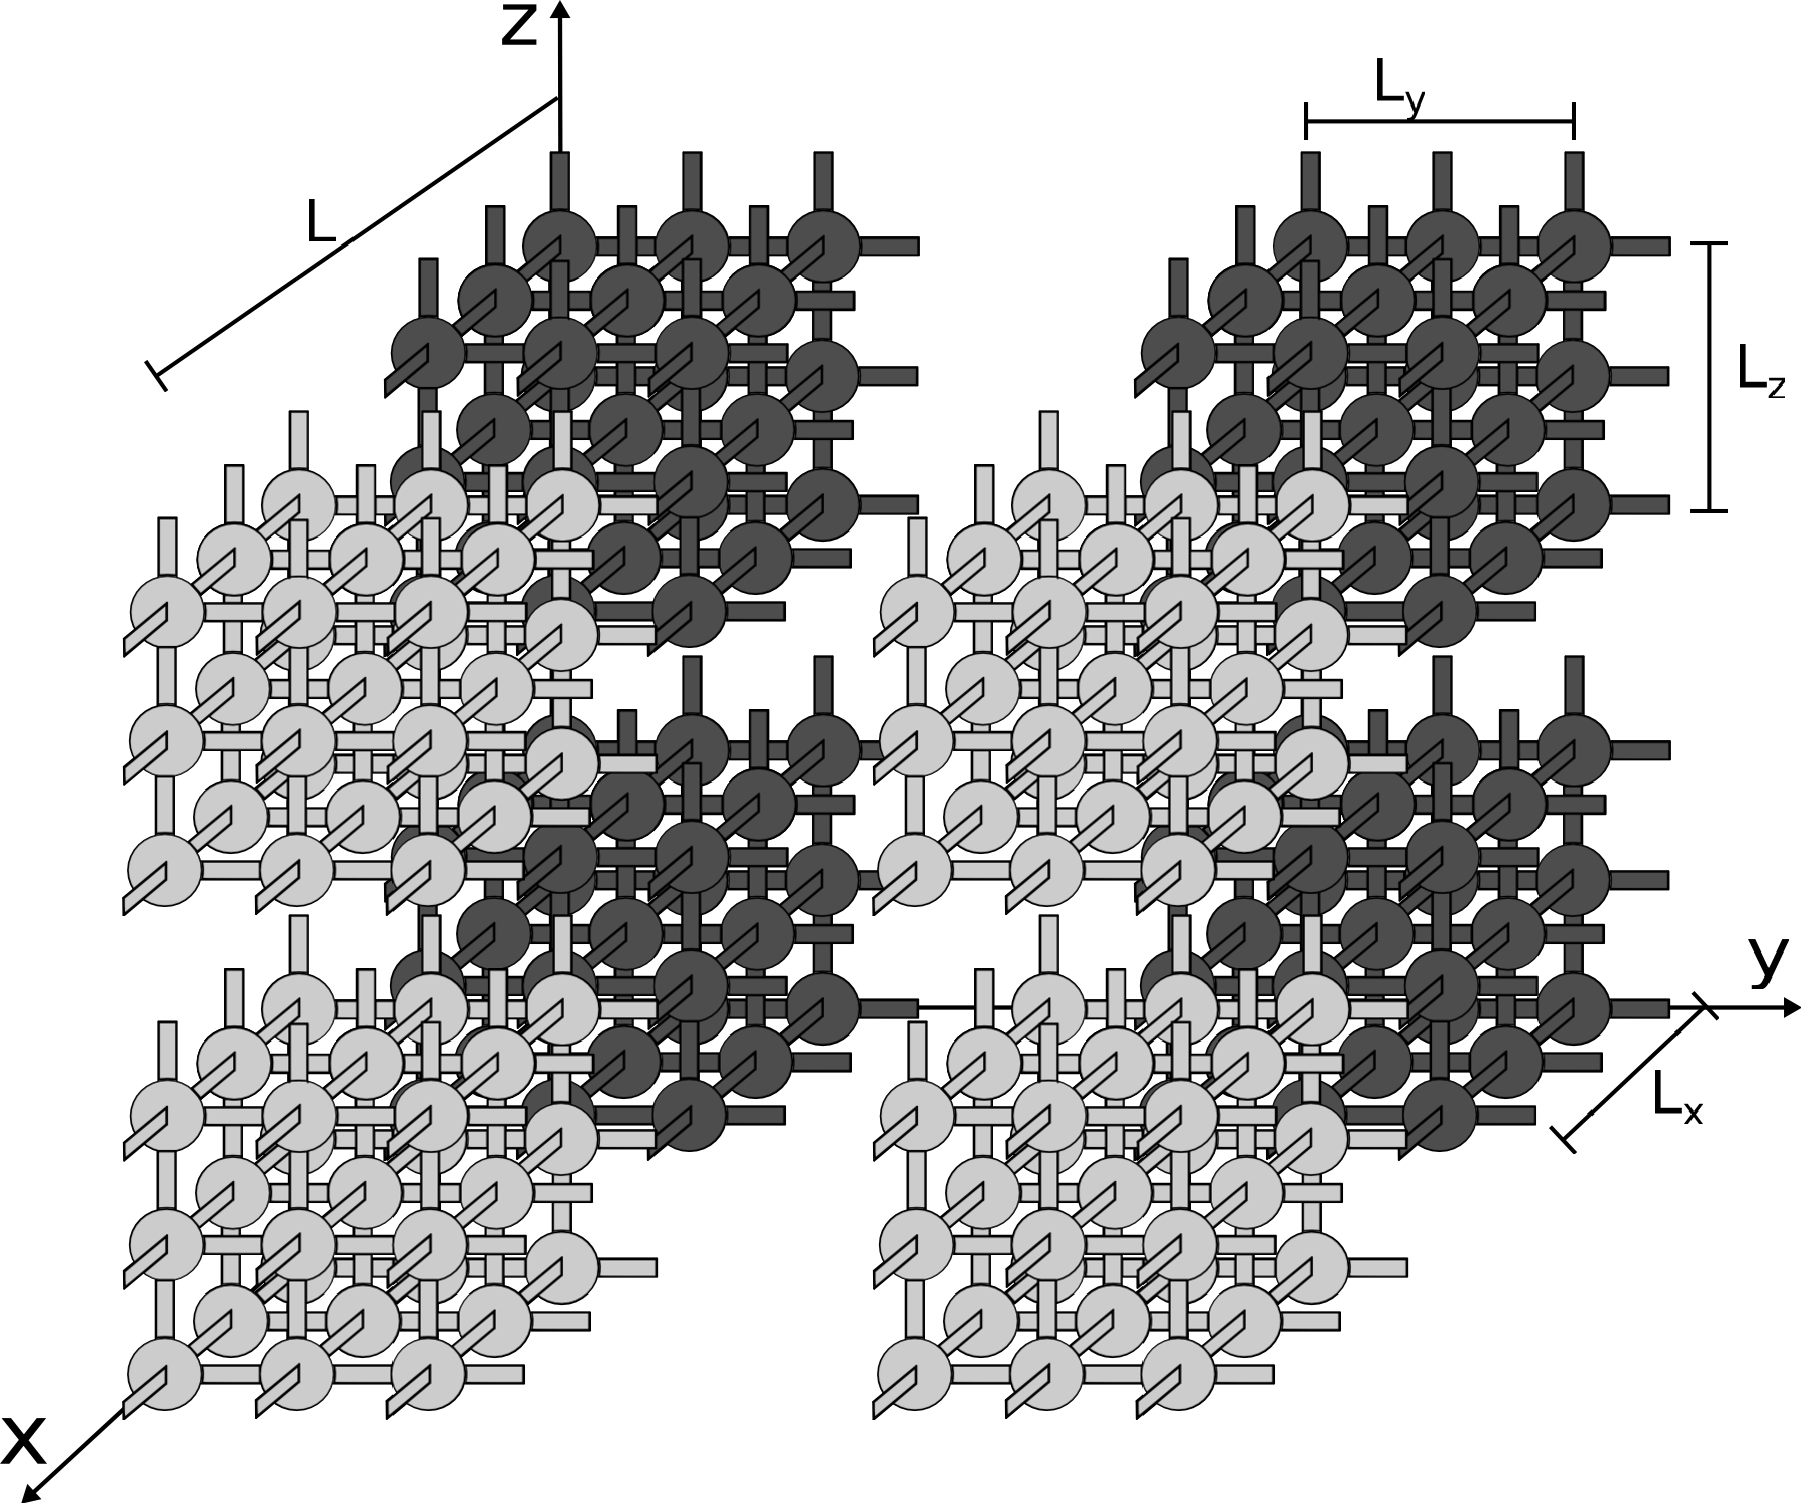
\includegraphics[width=2.8in]{img/distribucion}
\caption{Distribución de una red porosa entre 8 procesos MPI}
\label{fig:distribucion_rw}
\end{figure}


\subsubsection{Algoritmo Paralelo S-NoMISS}
\label{subsubsec:ps-nomiss}
El algoritmo paralelo S-NoMISS se describe con mayor detalle en \cite{ref3}, y esta basado en el algoritmo NoMISS descrito en la sección anterior adicionalmente al ser un algoritmo paralelo este utiliza una método estático para la distribución de carga, lo pasos del algoritmo son los siguientes:

\begin{enumerate}
\item \textbf{Generación de poros}: Cada nodo generará $L^3/N$ sitios y $3L^3/N$ enlaces, donde $N$ es el número de nodos a utilizar, los sitios se ordenan de forma ascendente(Parallel-Quicksort). Y cada nodo crea las listas locales $L_S$ y $L_{SC}$ basándose en el paso 1 del algoritmo NoMISS.

\item \textbf{Sembrado}: Cada nodo ejecuta sobre su subred el paso 2 del algoritmo NoMISS secuencial. Con la restricción de que se omiten las caras externas de cada subred.

\item \textbf{Rellenado}: Para lograr cumplir el $PC$ entre las fronteras de las subredes adyacentes y rellenar los espacios vacíos existentes entre estas, se realizan un serie de trasferencias a lo largo de los ejes $x$, $y$ y $z$ entre las subredes vecinas para que de esta forma se generan subredes temporales que toman en cuenta las fronteras de cada subred. En las subredes temporales se siguen asignado sitios y enlaces en los espacios vacíos. Al terminar los pasos 2 y 3 se tiene una red porosa válida.
\end{enumerate}

\subsubsection{Algoritmo Paralelo D-NoMISS}
\label{subsubsec:pd-nomiss}
El algoritmo paralelo D-NoMISS se describe con mayor detalle en \cite{ref4}, este algoritmo ejecuta los pasos del algoritmo S-NoMISS con algunas modificaciones. Los pasos que cambian respecto al algoritmo secuencial NoMISS son los pasos 2 y 3:

\begin{enumerate}
\item \textbf{Generación de poros}: paso 1 de S-NoMISS

\item \textbf{Sembrado paralelo}: El sembrado inicial de forma normal como en NoMISS omitiendo las caras externas de cada subred, las semillas y los clusters ocupan hasta el $25\%$ de la subred. Para que cada poro tenga la posibilidad de ser sembrado al inicio, cada nodo trasfiere la mitad de la subred a los vecinos($x$, $y$ y $z$), por cada trasferencia se realiza una siembra paralela. Cabe destacar que las listas $L_{SC}$ locales de cada nodo no son necesariamente del mismo tamaño al final de la siembra

\item \textbf{Rellenado paralelo}: Cada nodo intenta llenar los lugares vacíos de su subred mediante un cluster que se extiende hasta un tamaño $(L_x -2) \cdot (L_y - 2) \cdot (L_z -2)$, excluyendo las caras externas de la subred. Debido al paso dos y las posibilidad de que las listas $L_{SC}$ sean de distintos tamaños se genera una política de distribución de carga que hace que las listas permanezcan equilibradas.
\end{enumerate}

En todos los algoritmos descritos en este capítulo se recomienda aplicar un número adicional de $MCs$ para mejorar la isotropía de la red porosa ya sea de forma secuencial o paralela.\\

%\section{Computo paralelo sobre memoria compartida}
%\label{sec:rwconclutions}

\section{Resumen}
\label{sec:rwconclutions}
En general los algoritmos NoMISS tienen un mejor rendimiento que los algoritmos BiaSED, especialmente cuando se pretende construir redes porosas con alto traslape ($\Omega$). En cuanto a las versiones paralelas de NoMISS la versión S-NoMISS se observa mejor en términos de tiempo; sin embargo en términos de la ísotropía de la red el algoritmo D-NoMISS es mejor, el mayor problema de la versión D-NoMISS es que su método de distribución dinámica genera un cuello de botella que hace que su escalabilidad sea limitada. Las versiones paralelas existentes se toman únicamente como antecedentes y no como un punto de partida o comparación ya que en el presente trabajo se muestra una nuevo método para la construcción redes porosas  más reales el cual toma en cuenta nuevos parámetros que los algoritmos paralelos actuales no.\\

Se implemento y se evaluó una versión para crear redes de poros que cumplan con las $RG$, en la cual se replico el algoritmo secuencial de NoMISS para que cumpliese con las $RG$, sin embargo debido a que los enlaces y sitios se generan de forma aleatoria era muy difícil encontrar configuraciones válidas lo que se trasformaba en tiempos de ejecución muy altos y como resultado solo se logro generar redes de porosas con traslapes muy pequeños ($\Omega<=0.0007$) utilizando este esquema, en base al resultado anterior no se intento paralelizar dicha versión ya que la limitante del traslape afectaría de igual forma a una versión paralela. Para resolver este problema en los Capítulos \ref{champ:BSGR} y \ref{champ:PBSGR} proponemos una nueva solución para la construcción de redes prosas más reales tomando como base las Restricciones Geométricas. En nuestra versión paralela pretendemos sacar el mayor provecho de las arquitecturas multi-núcleo y los beneficios de la memoria compartida.



